\documentclass{standalone}
\usepackage{tikz}
\usepackage{ctex,siunitx}
\setCJKmainfont{Noto Serif CJK SC}
\usepackage{tkz-euclide}
\usepackage{amsmath}
\usetikzlibrary{patterns, calc,3d}
\usetikzlibrary {decorations.pathmorphing,decorations.pathreplacing,decorations.shapes,}
\begin{document}
\small
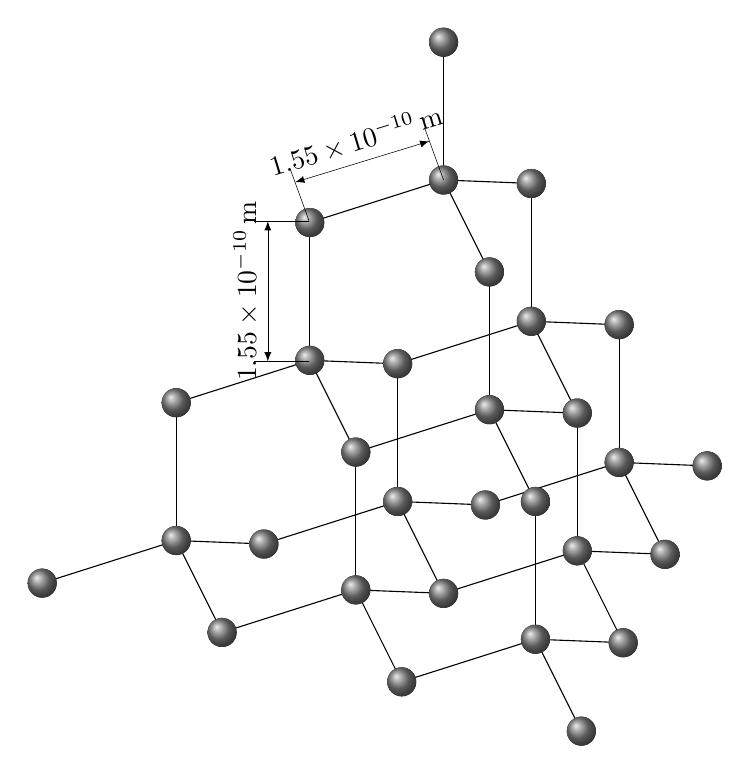
\begin{tikzpicture}[>=latex,scale=3.5]
  \begin{scope}[z={(10:10mm)},x={(-45:5mm)}]
  \foreach \x/\y/\z in { 0.000/ 0.000/ 0.000,-0.236/-0.667/-0.408,-0.471/-1.333/-0.816, 0.236/-1.333/-0.408, 0.471/-0.667/ 0.000, 0.943/-1.333/ 0.000, 0.236/-1.333/ 0.408,-0.236/-0.667/ 0.408,-0.471/-1.333/ 0.000,-0.471/-1.333/ 0.816}
  {
    \draw(\x,\y,\z)--++(0,0.5,0);
    \draw(\x,\y,\z)--++(-0.2357,-0.1667,-0.4082);
    \draw(\x,\y,\z)--++(-0.2357,-0.1667,0.4082);
    \draw(\x,\y,\z)--++(0.4714,-0.1667,0.0000);
    \fill[ball color=gray](\x,\y,\z)circle(1.5pt);
  }
  \foreach \x/\y/\z in{ 0.000/ 0.500/ 0.000,-0.236/-0.167/-0.408,-0.471/-0.833/-0.816,-0.707/-1.500/-1.225,-0.707/-1.500/-0.408,-0.707/-1.500/ 0.408,-0.707/-1.500/ 1.225,-0.471/-0.833/ 0.000, 0.236/-0.833/ 0.408, 0.000/-1.500/ 0.000, 0.707/-1.500/ 0.408, 1.414/-1.500/ 0.000, 0.943/-0.833/ 0.000, 0.000/-1.500/ 0.816, 0.471/-0.167/ 0.000, 0.236/-0.833/-0.408,-0.236/-0.167/ 0.408, 0.000/-1.500/-0.816,-0.471/-0.833/ 0.816,0.707/-1.500/-0.408}
  { \fill[ball color=gray](\x,\y,\z)circle(1.5pt); }
\end{scope}
\draw[very thin](0,0)--(110:0.2)(-163:0.51)--++(110:0.2);
\draw[very thin,<->](110:0.15)--++(-163:0.51)node[midway,sloped,above]{\qty{1.55e-10}{m}};
\draw[very thin](-163:0.51)--++(180:0.2)([yshift=-5.1mm]-163:0.51)--++(180:0.2);
\draw[very thin,<->]([xshift=-1.5mm]-163:0.51)--++(270:0.51)node[midway,sloped,above,rotate=180]{\qty{1.55e-10}{m}};
\end{tikzpicture}
\end{document}